\documentclass[11pt]{article} \usepackage{october} \onehalfspacing

\begin{document}

\textbf{Synopsis}

In the early 1970s, the dominant models for similarity in the
psychological literature were all geometric in nature. Distance
measures capturing similarity and dissimilarity between concepts
obeyed minimality, symmetry, and the triangle inequality. Then Amos
Tversky wrote a compelling paper, \qeins{Features of Similarity,}
undermining the idea that a metric topology is the best model. Tversky
gave both theoretical and empirical reasons why similarity between
concepts did not fulfill minimality, symmetry, or the triangle
inequality. Geometry with its metric distance measures was not a
helpful way to model similarity. Tversky presented an alternative
set-theoretic approach which accommodated the data that could not be
reconciled with a geometry of similarity.

The aim of this paper is to help along a similar paradigm shift when
it comes to epistemic modeling of closeness or difference between
subjective probability distributions. The geometry of reason (a term
coined by Richard Pettigrew and Hannes Leitgeb, two of its advocates)
also violates reasonable expectations we may have toward an acceptable
model. Just as Tversky did, I will present a non-geometric and
asymmetric alternative: information theory. Information theory
fulfills the expectations that the geometry of reason violates and
incorporates basic Bayesian commitments to probabilism and standard
conditioning.

The epistemic utility approach in Bayesian epistemology has attracted
some attention in the past few years. James Joyce, in an article
programmatically named \qeins{A Nonpragmatic Vindication of
  Probabilism,} defends probabilism supported by partial-belief-based
epistemic utility rather than the pragmatic utility common in
Dutch-book style arguments. For Joyce, norms of gradational accuracy
characterize the epistemic utility approach to partial beliefs,
analogous to norms of truth for full beliefs.

Richard Pettigrew and Hannes Leitgeb have published arguments that
under certain assumptions probabilism and standard conditioning (which
together give epistemology a distinct Bayesian flavour) minimize
inaccuracy, thereby providing maximal epistemic utility. Leitgeb and
Pettigrew show, given the geometry of reason and other axioms inspired
by Joyce (for example normality and dominance), that in order to avoid
epistemic dilemmas we must commit ourselves to a Brier score measure
of inaccuracy and subsequently to probabilism and standard
conditioning. Jeffrey conditioning (also called probability
kinematics) is widely considered to be a commonsense extension of
standard conditioning. On Leitgeb and Pettigrew's account, it fails to
provide maximal epistemic utility. Another type of conditioning, which
we will call LP conditioning, takes the place of Jeffrey conditioning.

The failure of Jeffrey conditioning to minimize inaccuracy on the
basis of the geometry of reason casts, by reductio, doubt on the
geometry of reason. I will show that LP conditioning, which the
geometry of reason entails, fails seven commonsense expectations that
are reasonable to have for the kind of updating scenario that LP
conditioning addresses. Leitgeb and Pettigrew do little to
substantiate a link between the geometry of reason and epistemic
utility on a conceptual level. It is the formal success of the model
that makes the geometry of reason attractive, but the failure of LP
conditioning to meet basic expectations undermines this success.

The question then remains whether we have a plausible candidate to
supplant the geometry of reason. The answer is yes: information theory
provides us with a measure of closeness between probability
distributions on a finite event space that has more conceptual appeal
than the geometry of reason, especially with respect to epistemic
utility---it is intuitively correct to relate updating to exchange of
information. More persuasive than intuitions, however, is the fact
that information theory supports both standard conditioning and the
extension of standard conditioning to Jeffrey conditioning, an
extension which is formally continuous with the standard conditioning
which Leitgeb and Pettigrew have worked so hard to vindicate
nonpragmatically. LP conditioning is not continuous with standard
conditioning---one of the seven expectations that LP conditioning
fails to meet. The other six, in brief, concern regularity (avoiding
extreme probabilities when not required by the evidence); a scenario
introduced by Benjamin Levinstein in a recent paper; an invariance
failure; dissonance with confirmation theory; an analogy with event
horizons; and, more controversially, asymmetry.

Leitgeb and Pettigrew's reasoning to establish LP conditioning on the
basis of the geometry of reason is valid. Given the failure of LP
conditioning to fulfill the seven expectations, it cannot be sound.
The premise to reject is the geometry of reason. Fortunately,
information theory replaces it and yields results that fulfill the
seven expectations, although I also note in the paper that the burden
is on information theory to give an epistemic justification explaining
the non-trivial structure of its symmetry breaking.

\newpage

\section{Introduction}
\label{intr}

The geometry of reason refers to a view of epistemic utility in which
the underlying topology for credence functions (which may be
subjective probability distributions) on a finite number of events is
a metric space. Since the isomorphism is to a metric space, there is a
distance relation between credence functions which can be used to
formulate axioms relating credences to epistemic utility and to
justify or to criticize contentious positions such as Bayesian
conditionalization, the principle of indifference, other forms of
conditioning, or probabilism itself (see especially works cited below
by James Joyce; Pettigrew and Leitgeb; David Wallace and Hilary
Greaves).

My claim is that given an epistemic utility approach and some
intuitive axioms, the geometry of reason leads itself ad absurdum; and
that there is a viable alternative to the geometry of reason which
avoids the problematic implications: information theory. For
information theory, as opposed to the geometry of reason, the
underlying topology for credence functions is not a metric space (see
figures \ref{fig:contourslp} and \ref{fig:contoursrj} for
illustration).

\begin{figure}[ht]
  \begin{flushright}
    \begin{minipage}[h]{.7\linewidth}
      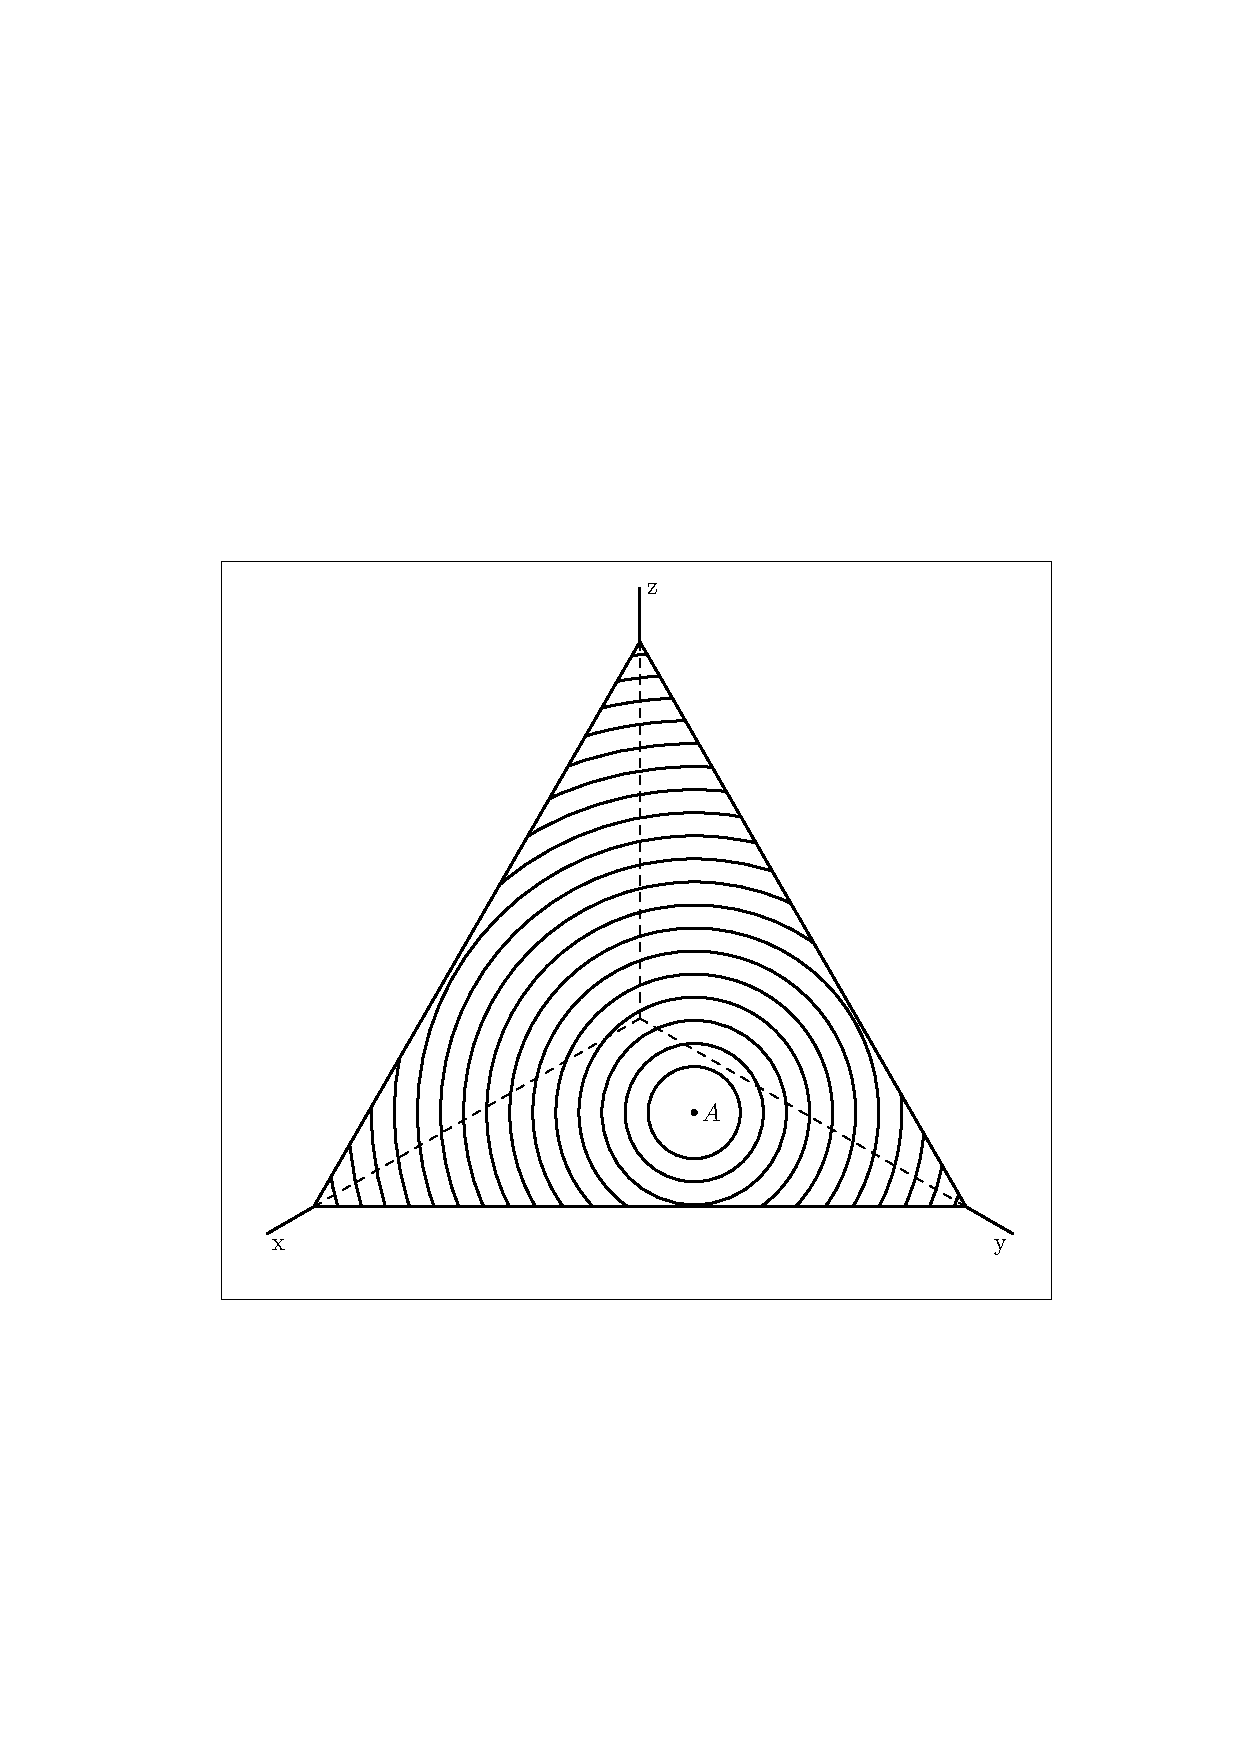
\includegraphics[width=\textwidth]{contourslp.pdf}
      \caption{\footnotesize The simplex $\mathbb{S}^{3}$ in
        three-dimensional space $\mathbb{R}^{3}$ with contour lines
        corresponding to the geometry of reason around point $A$ in
        equation (\ref{eq:e6}). Points on the same contour line are
        equidistant from $A$ with respect to the Euclidean metric.
        Compare the contour lines here to figure
        (\ref{fig:contoursrj}). Note that this diagram and all the
        following diagrams are frontal views of the simplex.}
      \label{fig:contourslp}
    \end{minipage}
  \end{flushright}
\end{figure}

\begin{figure}[ht]
  \begin{flushright}
    \begin{minipage}[h]{.7\linewidth}
      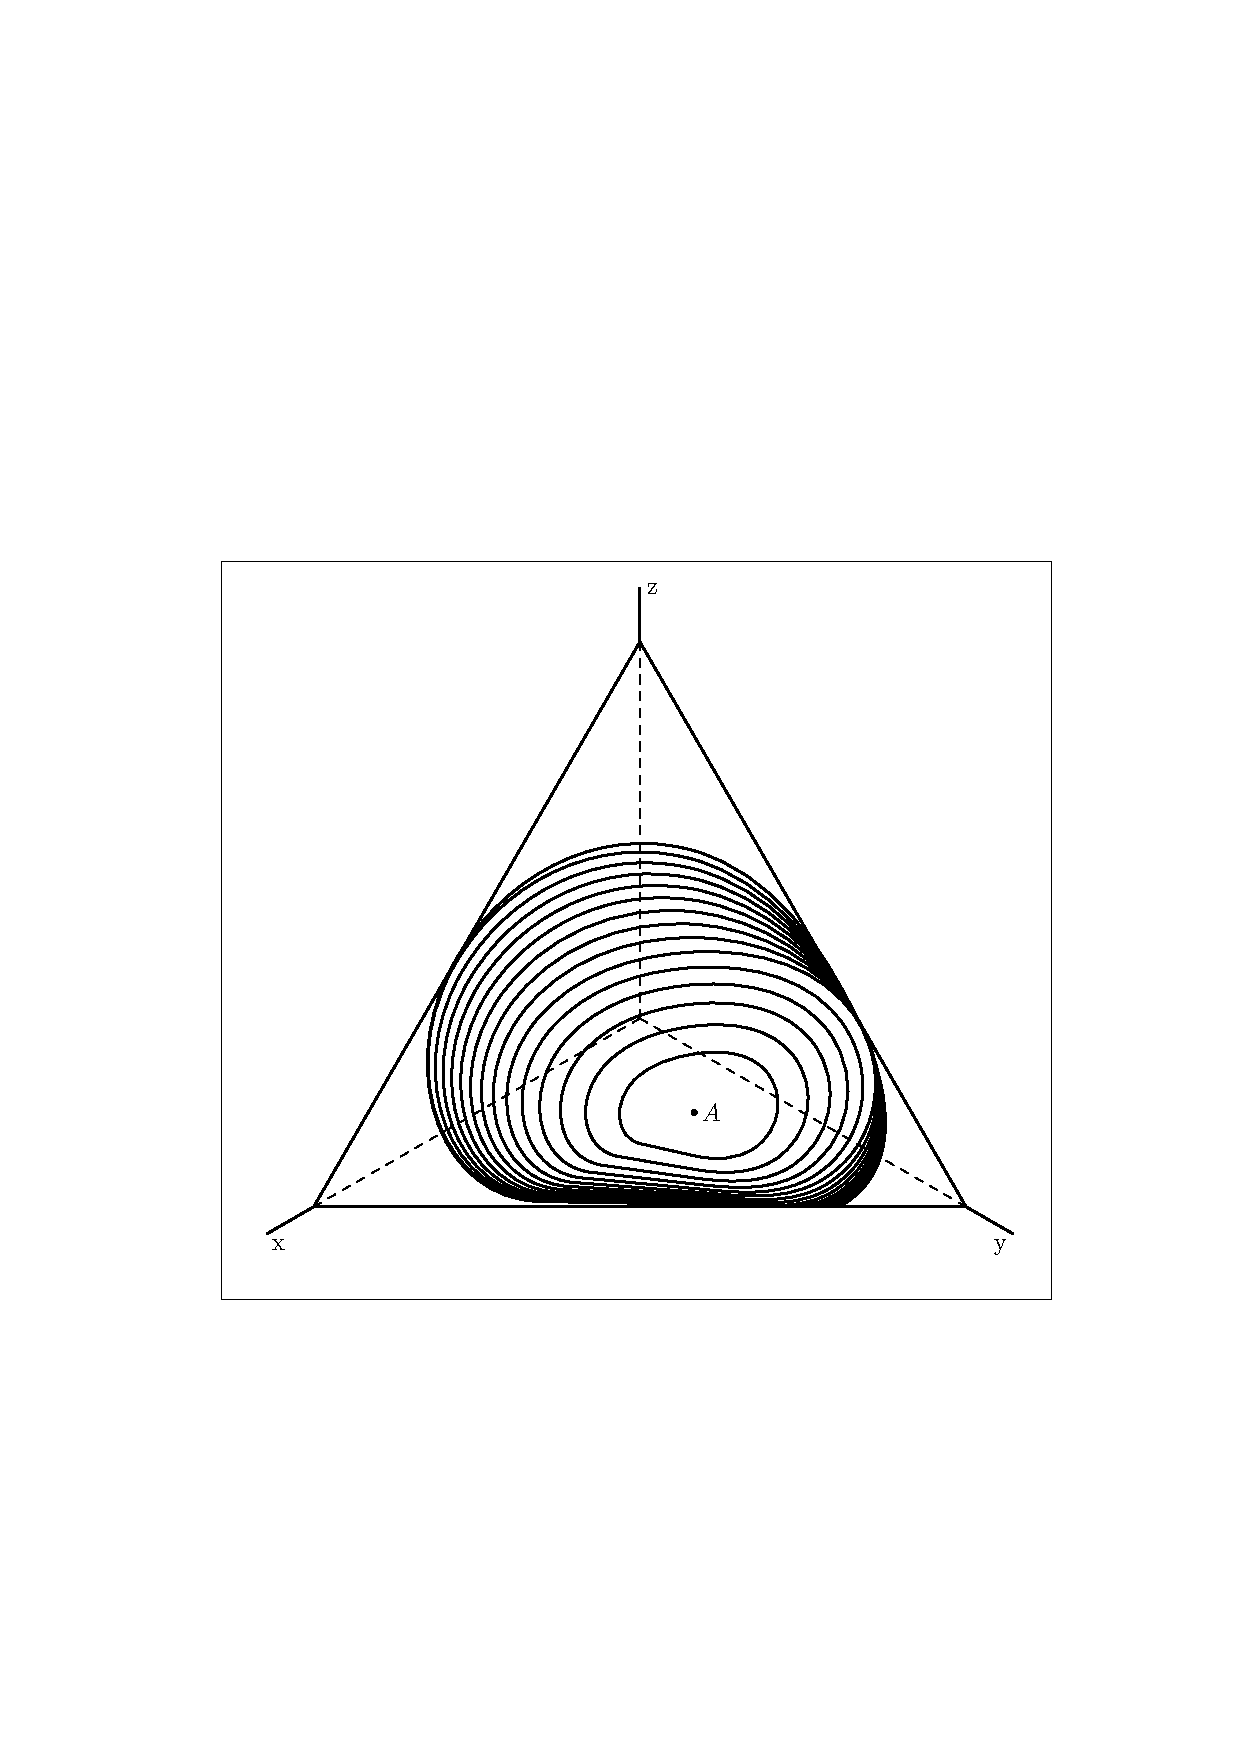
\includegraphics[width=\textwidth]{crj.pdf}
      \caption{\footnotesize The simplex $\mathbb{S}^{3}$ with contour
        lines corresponding to information theory around point $A$ in
        equation (\ref{eq:e6}). Points on the same contour line are
        equidistant from $A$ with respect to the Kullback-Leibler
        divergence. The contrast to figure (\ref{fig:contourslp}) will
        become clear in much more detail in the body of the paper.
        Note that the contour lines of the geometry of reason are
        insensitive to the boundaries of the simplex, while the
        contour lines of information theory reflect them. The main
        argument of this paper is that information theory respects
        epistemic intuitions we have about asymmetry: proximity to
        extreme beliefs with very high or very low probability
        influences the topology that is at the basis of updating.}
      \label{fig:contoursrj}
    \end{minipage}
  \end{flushright}
\end{figure}

\section{Epistemic Utility and the Geometry of Reason}
\label{eugr}

Joyce advocates for axioms such as Weak Convexity and Symmetry in
Euclidean terms, using justifications such as \qeins{the change in
  belief involved in going from $b'$ to $b''$ has the same direction
  but a doubly greater magnitude than change involved in going from
  $b'$ to [the midpoint] $m$} (see \scite{8}{joyce98}{596}). Terms
such as \qnull{midpoint} between two distributions and
$\lambda{}b'+(1-\lambda)b''$ for distributions \qnull{between} two
distributions $b'$ and $b''$ are used freely.

Leitgeb and Pettigrew muse about alternative geometries, especially
non-Euclidean ones. They suspect that these would be based on and in
the end reducible to Euclidean geometry but they do not entertain the
idea that they could drop the requirement of a metric topology
altogether (for the use of non-Euclidean geodesics in statistical
inference see \scite{7}{shunichi85}{}).

Leitgeb and Pettigrew's work is continuous with Joyce's work, although
their axioms tend to be stronger including expected inaccuracies. They
show that uniform distribution (a version of the principle of
indifference) requires additional axioms which are much less plausible
than the ones on the basis of which they derive probabilism and
standard conditioning (see \scite{8}{leitgebpettigrew10ii}{250f}); and
that Jeffrey conditioning does not fulfill Joyce's Norm of Gradational
Accuracy (see \scite{8}{joyce98}{579}). Leitgeb and Pettigrew provide
us with an alternative method of updating for Jeffrey-type updating
scenarios, which I will call LP conditioning.

\begin{quotex}
  \beispiel{Sherlock Holmes}\label{ex:holmes} Sherlock Holmes
  attributes the following probabilities to the propositions $E_{i}$
  that $k_{i}$ is the culprit in a crime:
  $P(E_{1})=1/3,P(E_{2})=1/2,P(E_{3})=1/6$, where $k_{1}$ is Mr.\ R.,
  $k_{2}$ is Ms.\ S., and $k_{3}$ is Ms.\ T. Then Holmes finds some
  evidence which convinces him that $P'(F^{*})=1/2$, where $F^{*}$ is
  the proposition that the culprit is male and $P$ is relatively prior
  to $P'$. What should be Holmes' updated probability that Ms.\ S. is
  the culprit?
\end{quotex}

I will look at the recommendations of Jeffrey conditioning and LP
conditioning for example \ref{ex:holmes} in the next section. For now,
we note that LP conditioning violates all of the following seven
plausible expectations for an amujus, an \qnull{alternative method of
  updating for Jeffrey-type updating scenarios.} Example
\ref{ex:holmes} is just such an amujus.

\begin{itemize}
\item \textsc{continuity} An amujus ought to be continuous with
  standard conditioning as a limiting case.
\item \textsc{regularity} An amujus ought not to assign a posterior
  probability of $0$ to an event which has a positive prior
  probability and about which the intervening evidence says nothing
  except that a strictly weaker event has a positive posterior
  probability.
\item \textsc{levinstein} An amujus ought not to give \qeins{extremely
    unattractive} results in a Levinstein scenario (see
  \scite{7}{levinstein12}{}).
\item \textsc{invariance} An amujus ought to be partition invariant.
\item \textsc{horizon} An amujus ought to exhibit the horizon effect
  which makes probability distributions which are nearer to extreme
  probability distributions appear to be closer to each other than
  they really are.
\item \textsc{confirmation} An amujus ought to align with intuitions
  we have about degrees of confirmation.
\item \textsc{asymmetry} An amujus ought to reflect epistemic
  asymmetries. Updating from one probability distribution to another
  may need to be reflected in a different proximity relation than
  going the opposite way.
\end{itemize}

We are faced with the choice of rejecting the geometry of reason or
accepting these unpleasant consequences. Fortunately, there is a live
alternative to the geometry of reason: information theory. Information
theory has its own axiomatic approach to justifying probabilism and
standard conditioning (see \scite{7}{shorejohnson80}{}). Furthermore,
information theory provides a justification for Jeffrey conditioning
and generalizes it (see \scite{7}{lukits15}{}).

Information theory, as opposed to the geometry of reason, measures
divergences, not distances, between distributions of partial belief.
The term \qnull{information geometry} is therefore a bit of an
oxymoron. It is due to Imre Csisz{\'a}r, who considers the
Kullback-Leibler divergence an asymmetric analogue of squared
Euclidean distance and derives several results that are intuitive
information geometric counterparts of standard results in Euclidean
geometry (see chapter 3 of \scite{7}{csiszarshields04}{}). The
divergence of $b''$ from $b'$ may not be equal to the divergence of
$b'$ from $b''$. Updating methods based on information theory
(standard conditioning, Jeffrey conditioning, the principle of maximum
entropy) fulfill the seven expectations.

\section{Geometry of Reason versus Information Theory}
\label{grit}

Consider the following three points in three-dimensional space:

\begin{equation}
  \label{eq:e6}
  A=\left(\frac{1}{3},\frac{1}{2},\frac{1}{6}\right) \hspace{.5in}
  B=\left(\frac{1}{2},\frac{3}{8},\frac{1}{8}\right)  \hspace{.5in}
  C=\left(\frac{1}{2},\frac{5}{12},\frac{1}{12}\right)
\end{equation}

All three are elements of the three-dimensional simplex
$\mathbb{S}^{3}$: their coordinates add up to $1$. Thus they represent
probability distributions over a partition of the event space into
three events. Now call $D_{\mbox{\tiny KL}}(A,B)$ the Kullback-Leibler
divergence of $A$ from $B$ defined as follows, where $a_{i}$ are the
Cartesian coordinates of $A$:

\begin{equation}
  \label{eq:e7}
  D_{\mbox{\tiny KL}}(A,B)=\sum_{i=1}^{3}a_{i}\ln\frac{a_{i}}{b_{i}}
\end{equation}

The Euclidean distance $\|A-B\|$ is defined as

\begin{equation}
  \label{eq:e3}
  \sqrt{\sum_{i=1}^{3}\left(a_{i}-b_{i}\right)^{2}}.
\end{equation}

What is remarkable about the three points in (\ref{eq:e6}) is that

\begin{equation}
  \label{eq:e8}
  \|A-C\|\approx{}0.204<\|A-B\|\approx{}0.212
\end{equation}

and

\begin{equation}
  \label{eq:e9}
  D_{\mbox{\tiny KL}}(A,B)\approx{}0.057<D_{\mbox{\tiny KL}}(A,C)\approx{}0.072.
\end{equation}

The Kullback-Leibler divergence and Euclidean distance give different
recommendations with respect to proximity (for illustration see figure
\ref{fig:threepoints}). If $A$ corresponds to my prior and my evidence
is such that I must change the first coordinate to $1/2$ and nothing
stronger, then information theory via the Kullback-Leibler divergence
recommends the posterior corresponding to $B$, whereas the geometry of
reason recommends the posterior corresponding to $C$.

\begin{figure}[ht]
  \begin{flushright}
    \begin{minipage}[h]{.7\linewidth}
      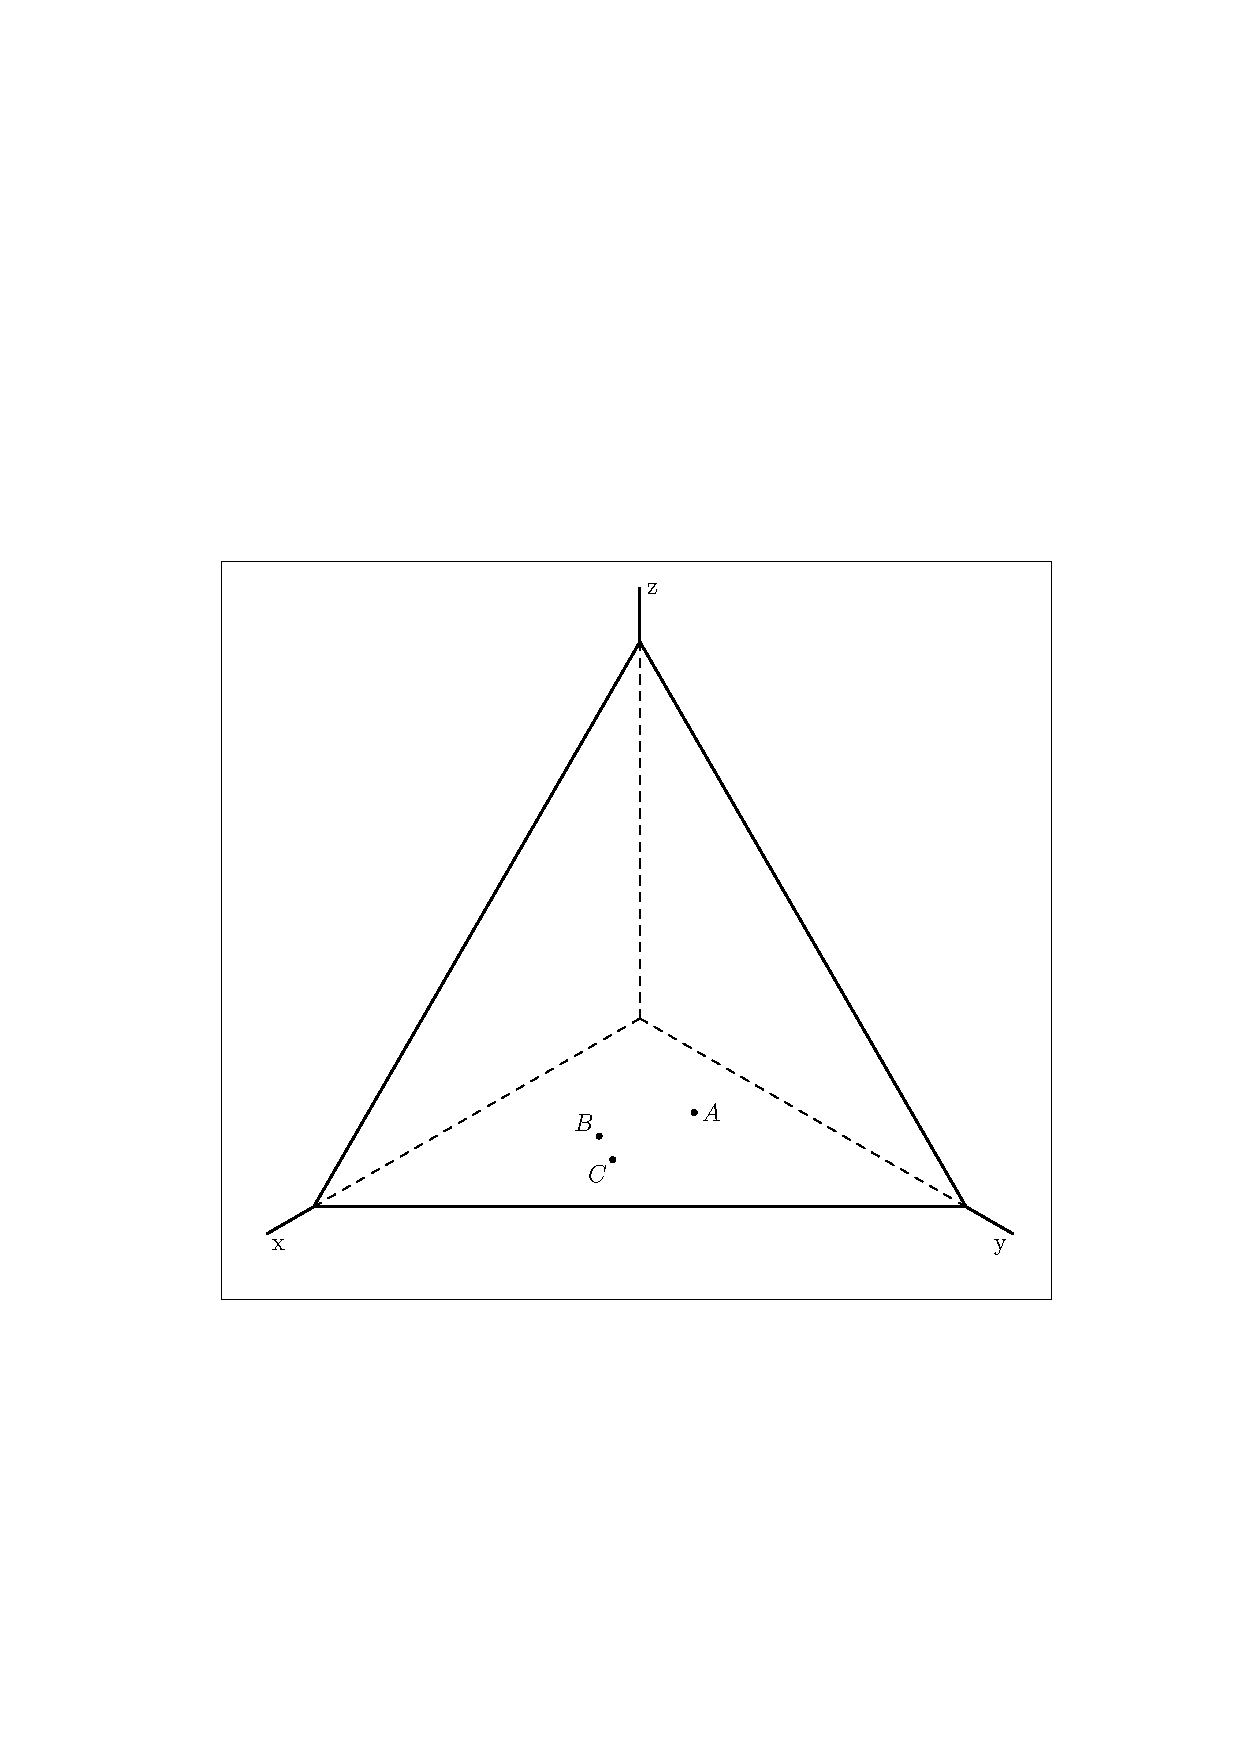
\includegraphics[width=\textwidth]{threepoints.pdf}
      \caption{\footnotesize The simplex $\mathbb{S}^{3}$ in
        three-dimensional space $\mathbb{R}^{3}$ with points $A,B,C$
        as in equation (\ref{eq:e6}). Note that geometrically speaking
        $C$ is closer to $A$ than $B$ is. Using the Kullback-Leibler
        divergence, however, $B$ is closer to $A$ than $C$ is. The
        reason is asymmetry in information theory, which accords with
        our intuitions about epistemic space.}
      \label{fig:threepoints}
    \end{minipage}
  \end{flushright}
\end{figure}

Here is a brief outline how Leitgeb and Pettigrew arrive at posterior
probability distributions in Jeffrey-type updating scenarios, using
their invariance criterion with respect to global and local
inaccuracy. I will call their method LP conditioning.

\begin{quotex}
  \beispiel{Abstract Holmes}\label{ex:abstract} Consider a possibility
  space $W=E_{1}\cup{}E_{2}\cup{}E_{3}$ (the $E_{i}$ are sets of
  states which are pairwise disjoint and whose union is $W$) and a
  partition $\mathcal{F}$ of $W$ such that
  $\mathcal{F}=\{F^{*},F^{**}\}=\{E_{1},E_{2}\cup{}E_{3}\}$.
\end{quotex}

Let $P$ be the prior probability function on $W$ and $P'$ the
posterior. Jeffrey-type updating scenarios give us new information on
the posterior probabilities of partitions such as $\mathcal{F}$. In
example \ref{ex:abstract}, let

\begin{equation}
  \label{eq:priors}
  \begin{array}{rcl}
    P(E_{1})&=&1/3 \\
    P(E_{2})&=&1/2 \\
    P(E_{3})&=&1/6
  \end{array}
\end{equation}

and the new evidence constrain $P'$ such that
$P'(F^{*})=1/2=P'(F^{**})$.

Jeffrey conditioning works on the intuition that the posterior
probabilities conditional on the partition elements equal the prior
probabilities conditional on the partition elements (since we have no
information in the evidence that they should have changed):

\begin{align}
  \label{eq:jc}
  &P'_{\mbox{\tiny JC}}(E_{i})&=&P'(E_{i}|F^{*})P'(F^{*})+P'(E_{i}|F^{**})P'(F^{**})\notag \\
  &&=&P(E_{i}|F^{*})P'(F^{*})+P(E_{i}|F^{**})P'(F^{**})
\end{align}

Jeffrey conditioning is controversial (for an introduction to Jeffrey
conditioning see \scite{7}{jeffrey65}{}; for its statistical and
formal properties see \scite{7}{diaconiszabell82}{}; for a pragmatic
vindication of Jeffrey conditioning see \scite{7}{armendt80}{}, and
\scite{7}{skyrms86}{}; for criticism see
\scite{7}{howsonfranklin94}{}). Information theory, however, supports
Jeffrey conditioning.

Leitgeb and Pettigrew show that Jeffrey conditioning does not in
general pick out the minimally inaccurate posterior probability
distribution. If the geometry of reason as presented in Leitgeb and
Pettigrew is sound, this would constitute a powerful criticism of
Jeffrey conditioning. Leitgeb and Pettigrew introduce an alternative
to Jeffrey conditioning, which we have called LP conditioning. It
proceeds as follows for example \ref{ex:abstract} and in general
provides the minimally inaccurate posterior probability distribution
in Jeffrey-type updating scenarios.

Solve the following two equations for $x$ and $y$:

\begin{equation}
  \label{eq:lpce}
  \begin{array}{rcl}
    P(E_{1})+x&=&P'(F^{*}) \\
    P(E_{2})+y+P(E_{3})+y&=&P'(F^{**})
  \end{array}
\end{equation}

and then set

\begin{equation}
  \label{eq:lpcf}
  \begin{array}{rcl}
    P'_{\mbox{\tiny LP}}(E_{1})&=&P(E_{1})+x \\
    P'_{\mbox{\tiny LP}}(E_{2})&=&P(E_{2})+y \\
    P'_{\mbox{\tiny LP}}(E_{3})&=&P(E_{3})+y
  \end{array}
\end{equation}

For the more formal and more general account see
\scite{8}{leitgebpettigrew10ii}{254}. The results for example
\ref{ex:abstract} are:

\begin{equation}
  \label{eq:lpcres}
  \begin{array}{rcl}
    P'_{\mbox{\tiny LP}}(E_{1})&=&1/2 \\
    P'_{\mbox{\tiny LP}}(E_{2})&=&5/12 \\
    P'_{\mbox{\tiny LP}}(E_{3})&=&1/12
  \end{array}
\end{equation}

Compare these results to the results of Jeffrey conditioning:

\begin{equation}
  \label{eq:jcres}
  \begin{array}{rcl}
    P'_{\mbox{\tiny JC}}(E_{1})&=&1/2 \\
    P'_{\mbox{\tiny JC}}(E_{2})&=&3/8 \\
    P'_{\mbox{\tiny JC}}(E_{3})&=&1/8
  \end{array}
\end{equation}

Note that (\ref{eq:priors}), (\ref{eq:jcres}), and (\ref{eq:lpcres})
correspond to $A,B,C$ in (\ref{eq:e6}).

\section{Seven Expectations}
\label{fivex}

It remains to provide more detail for the seven expectations and to
show how LP conditioning violates them. These subsections have been
abridged to accommodate the word limit for this submission. The
full-length paper contains the complete version of these arguments,
especially their formal components and examples.

\subsection{Continuity}
\label{Continuity}

LP conditioning violates \textsc{continuity} because standard
conditioning gives a different recommendation than a parallel sequence
of Jeffrey-type updating scenarios which get arbitrarily close to
standard event observation. This is especially troubling considering
how important the case for standard conditioning is to Leitgeb and
Pettigrew.

\subsection{Regularity}
\label{Regularity}

LP conditioning violates \textsc{regularity} because formerly positive
probabilities can be reduced to $0$ even though the new information in
the Jeffrey-type updating scenario makes no such requirements (as is
usually the case for standard conditioning). Ironically, Jeffrey-type
updating scenarios are meant to be a better reflection of real-life
updating because they avoid extreme probabilities.

The violation becomes especially egregious if we are already somewhat
sympathetic to an information-based account: the amount of information
required to turn a non-extreme probability into one that is extreme
($0$ or $1$) is infinite. Whereas the geometry of reason considers
extreme probabilities to be easily accessible by non-extreme
probabilities under new information (much like a marble rolling off a
table or a bowling ball heading for the gutter), information theory
envisions extreme probabilities more like an event horizon. The nearer
you are to the extreme probabilities, the more information you need to
move on. For an observer, the horizon is never reached.

\subsection{Levinstein}
\label{Levinstein}

LP conditioning violates \textsc{levinstein} because of \qeins{the
  potentially dramatic effect [LP conditioning] can have on the
  likelihood ratios between different propositions}
\scite{3}{levinstein12}{419}. Levinstein proposes a logarithmic
inaccuracy measure as a remedy to avoid violation of
\textsc{levinstein} (vaguely related to the Kullback-Leibler
divergence), but his account falls far short of the formal scope,
substance, and integrity of information theory. As a special case of
applying a Levinstein-type logarithmic inaccuracy measure, information
theory does not violate \textsc{levinstein}.

\subsection{Invariance}
\label{Invariance}

LP conditioning violates \textsc{invariance} because two agents who
have identical credences with respect to a partition of the event
space may disagree about this partition after LP conditioning, even
when the Jeffrey-type updating scenario provides no new information
about the more finely grained partitions on which the two agents
disagree.

\subsection{Horizon}
\label{Horizon}

\begin{quotex}
  \beispiel{Undergraduate Complaint}\label{ex:complaint} An
  undergraduate student complains to the department head that the
  professor will not reconsider an 89\% grade (which misses an A+ by
  one percent) when reconsideration was given to other students with a
  67\% grade (which misses a B- by one percent).
\end{quotex}

Intuitions may diverge, but the professor's reasoning is as follows.
To improve a 60\% paper by ten percent is easily accomplished: having
your roommate check your grammar, your spelling, and your line of
argument will sometimes do the trick. It is incomparably more
difficult to improve an 85\% paper by ten percent: it may take doing a
PhD to turn a student who writes the former into a student who writes
the latter. Consequently, the step from 89\% to 90\% is much greater
than the step from 67\% to 68\%.

The emphasis in this argument is on distance, not confirmation, but
the next subsection can be considered to be a special case of
\textsc{horizon}. LP conditioning violates \textsc{horizon} because it
ignores the epistemic intuition that proximity relations near extreme
probabilities are different than away from them (more central rather
than peripheral). It should be noted that there are non-Euclidean
metrics that obey both \textsc{horizon} and \textsc{confirmation}.

\subsection{Confirmation}
\label{Confirmation}

From an epistemic perspective, updating towards extreme probabilities
should become increasingly difficult. Once a hypothesis is already
considered to be highly likely or highly unlikely, confirmation or
disconfirmation is much harder to come by than in the case of
near-equiprobability between alternative hypotheses. The geometry of
reason ignores this analogy from confirmation theory; information
theory reflects it.

David Christensen's account of degree of confirmation, for example,
shows how $S$-support given by $E$ is stable over Jeffrey conditioning
on $\{E,\urcorner{}E\}$, which is not the case for LP-conditioning
(see \scite{8}{christensen99}{451}). LP conditioning violates
\textsc{confirmation}.

\subsection{Asymmetry}
\label{Asymmetry}

Asymmetry presents a problem for the geometry of reason as well as for
information theory. For the geometry of reason, the problem is akin to
\textsc{continuity}. For information theory, the problem is the
non-trivial nature of the asymmetries it induces, which somehow need
to be reconnected to epistemic justification. I will consider this
problem in a moment, but first I will have a look at the problem for
the geometry of reason.

Extreme probabilities are special and create asymmetries in updating:
moving in direction from certainty to uncertainty is asymmetrical to
moving in direction from uncertainty to certainty. Geometry of
reason's metric topology, however, allows for no asymmetries.

\begin{quotex}
  \beispiel{Extreme Asymmetry}\label{ex:extreme} Consider two cases
  where for case 1 the prior probabilities are
  $P(Y_{1})=0.4,P(Y_{2})=0.3,P(Y_{3})=0.3$ and the posterior
  probabilities are $P'(Y_{1})=0,P'(Y_{2})=0.5,P'(Y_{3})=0.5$; for
  case 2 the prior probabilities are
  $Q(Y_{1})=0,Q(Y_{2})=0.5,Q(Y_{3})=0.5$ and the posterior
  probabilities are $Q'(Y_{1})=0.4,Q'(Y_{2})=0.3,Q'(Y_{3})=0.3$;
\end{quotex}

Case 1 is a straightforward application of standard conditioning. Case
2 is much more complicated: what does it take to raise a prior
probability of zero to a positive number? In terms of information
theory, the information required is infinite. Case 2 is also not
compatible with standard conditioning (at least not with what Alan
H{\'a}jek calls the ratio analysis of conditional probability, see
\scite{7}{hajek03}{}). The geometry of reason may want to solve this
problem by signing on to a version of regularity, but then it may be
exposed to violating \textsc{regularity}.

Consider now the problem for information theory. Given the asymmetric
similarity measure of probability distributions that information
theory requires (the Kullback-Leibler divergence), a prior probability
distribution $P$ may be closer to a posterior probability distribution
$Q$ than $Q$ is to $P$ if their roles (prior-posterior) are reversed.
That is just what we would expect. The problem is that there is
another posterior probability distribution $R$ where the situation is
just the opposite: prior $P$ is further away from posterior $R$ than
prior $R$ is from posterior $P$. And whether a probability
distribution different from $P$ is of the $Q$-type or of the $R$-type
escapes any epistemic intuition.

Let me put this differently to emphasize the gravity of the situation
for information theory. For simplicity, let us consider probability
distributions and their associated credence functions on an event
space with three atoms $\Omega=\{\omega_{1},\omega_{2},\omega_{3}\}$.
The simplex $\mathbb{S}^{3}$ represents all of these probability
distributions. Every point $P$ in $\mathbb{S}^{3}$ representing a
probability distribution induces a partition on $\mathbb{S}^{3}$ into
points that are symmetric to $P$, positively skew-symmetric to $P$,
and negatively skew-symmetric to $P$ given the topology of information
theory.

In other words, if

\begin{equation}
  \label{eq:sksy}
  \Delta_{P}(P')=D_{\mbox{\tiny KL}}(P',P)-D_{\mbox{\tiny KL}}(P,P'),
\end{equation}

then, holding $P$ fixed, $\mathbb{S}^{3}$ is partitioned into three
regions, $\Delta^{-1}(\mathbb{R}_{>0})$ (red in figure
\ref{fig:concat}), $\Delta^{-1}(\mathbb{R}_{<0})$ (blue in figure
\ref{fig:concat}), and $\Delta^{-1}(\{0\})$ (in figure
\ref{fig:concat}, this would be the line between the red and the
blue). One could have a simple epistemic intuition such as \qnull{it
  takes less to update from a more uncertain probability distribution
  to a more certain probability distribution than the reverse
  direction,} where the degree of certainty in a probability
distribution is measured by its entropy. This simple intuition accords
with what we said about extreme probabilities: it is, ignoring
regularity for a moment, information-theoretically acceptable to
update by standard conditionalization, decreasing the entropy; but the
reverse direction is not covered by standard conditionalization and
requires an infinite amount of information (raising a zero probability
to a positive probability).

It turns out that the Kullback-Leibler divergence does not support
this simple intuition. The tripartite partition induced by
(\ref{eq:sksy}) is non-trivial---some probability distributions are of
the $Q$-type (red), some are of the $R$-type (blue), and it is
difficult to think of an epistemic distinction between them that does
not already presuppose information theory. See figure \ref{fig:concat}
for graphical illustration of this point.

\begin{figure}[ht]
  \begin{flushright}
    \begin{minipage}[h]{.82\linewidth}
      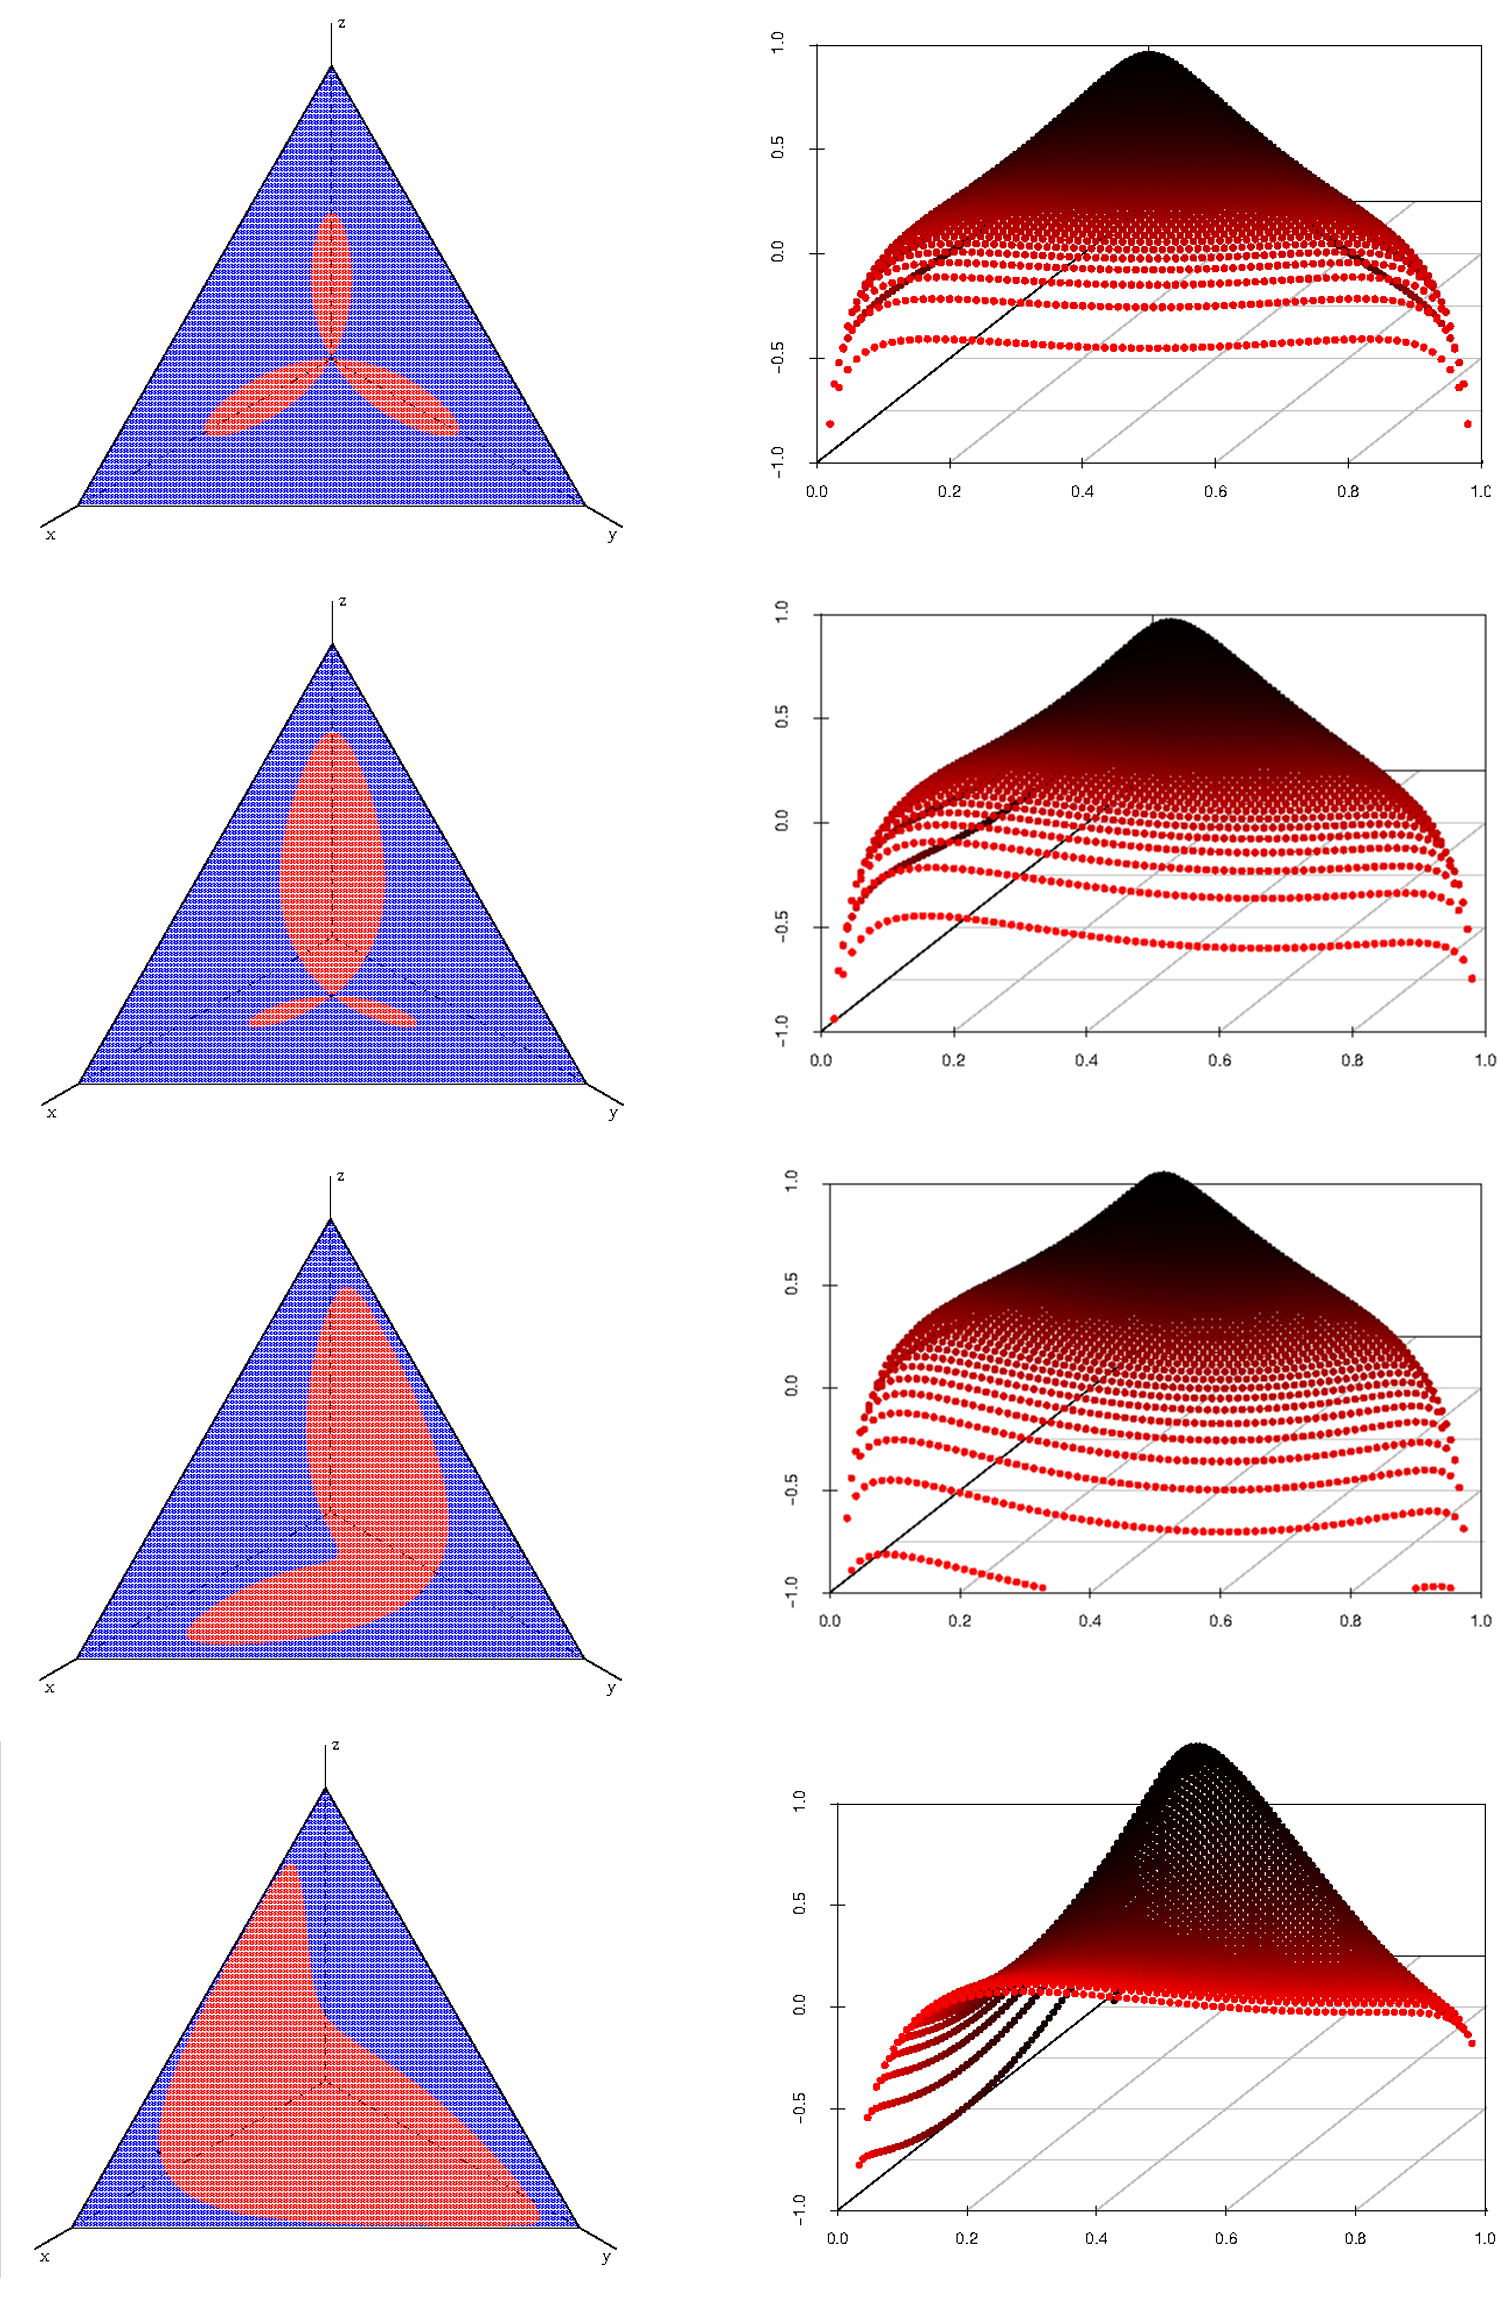
\includegraphics[width=\textwidth]{concat1.png}
      \caption{\footnotesize The partitions induced by equation
        (\ref{eq:sksy}) on the left, corresponding to the 3D
        scatterplot for $\Delta_{P}$ on the right. From top to bottom,
        $P=(1/3,1/3,1/3); P=(0.4,0.4,0.2); P=(0.242,0.604,0.154);
        P=(0.741,0.087,0.172)$.
        Note that for the geometry of reason, the diagrams are
        trivial. The challenge for information theory is to explain
        the non-triviality of these diagrams epistemically without
        begging the question.}
      \label{fig:concat}
    \end{minipage}
  \end{flushright}
\end{figure}

This paper has no solution for the problem which non-question-begging
epistemic explanation may justify the non-trivial asymmetries of
information theory. Yet I consider asymmetry to be much more plausible
than the symmetry that the geometry of reason advocates, even for
non-extreme probabilities. Less confidently than for the other six
expectations, I conclude that LP conditioning violates
\textsc{asymmetry}, and I add that an epistemic explanation of the
non-trivial asymmetries induced by information theory is needed.

\bibliographystyle{ChicagoReedweb} \bibliography{bib-2902}

\end{document}